% arara: lualatex
% !TEX TS-program = LuaLaTeX


% https://phys.libretexts.org/TextBooks_and_TextMaps/College_Physics/Book%3A_College_Physics_(OpenStax)/03._Two-Dimensional_Kinematics/3.4%3A_Projectile_Motion

\documentclass{coderdojo}

\worksheet{5}{Doing Physics with Python}

\newcommand\contentsitem[2]{
	\item \hyperref[#1]{\color{section}\bfseries #2}
}

\usepackage{wrapfig}

\newcommand\TODO[1]{
\begin{itemize}
\item[\todoSymbol] \color{todo} #1
\end{itemize}}


\begin{document}
\maketitle


\section*{Introduction}

In this worksheet we are going to do something a little different --- we are going to try and solve some real-world problems in Physics!  
In particular, we are going to look as {\bfseries projectile motion}. This is a part of Physics, which is interested in the movement of simple objects under the effect of gravity.  Don't worry if you have not covered these in school yet, most of this is just common sense and please ask us if we cover anything that is confusing.  

\vspace{24pt}
\centerline{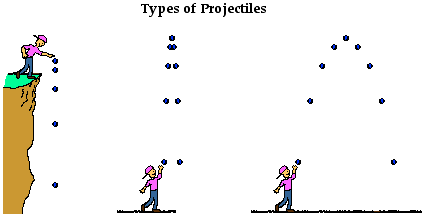
\includegraphics[width=.8\textwidth,clip,trim=0 0 0 20]{projectiles}}

\vspace{24pt}
As before we have broken up the task in separate stages:

\begin{dingautolist}{192}

\contentsitem{physics}{What are projectiles and what can I do with them?}

\contentsitem{drop}{Our First Experiment: Dropping a ball}

\contentsitem{drop}{Our Second Experiment: Throwing Up (without the mess!)}

\contentsitem{drop}{Visualising our projectiles}

\end{dingautolist}

And in the next worksheet we will look at 

\begin{dingautolist}{192}

\contentsitem{drop}{One Dimension is Boring, Lets go 2D}

\contentsitem{drop}{Generating graphs of the projectile movement.}

\end{dingautolist}


\clearpage

\section{Who asked for Physics?}

{\bfseries Projectile motion} is the motion of an object thrown or projected into the air, subject to only effect of gravity. The object is called a {\bfseries projectile}\footnote{If you can kick it, throw it or drop it then is is a projectile.}, and its path is called its {\bfseries trajectory}. We are interested in 

What do we know about moving objects? \ldots\ we know that we can calculate how fast we are moving by dividing the distance we have travelled by the length of time taken. So we have 

\begin{tcolorbox}
\begin{equation*}
	\text{velocity} = \frac{\text{distance}}{\text{time}}
	\qquad\iff\qquad
	\text{distance}
	= {\text{velocity}}\times {\text{time}}
\end{equation*}
\end{tcolorbox}

Lets think about this equation a bit to see if it make sense.  It says:
\begin{itemize}
\item
If velocity is larger (we are moving faster) then we will travel a larger distance. 
\dotfill \tickYes
\item
If time taken is larger then the distance travelled is larger
\dotfill \tickYes

\end{itemize}

Now since 
\[
	\text{distance} = (\text{new position}) - (\text{old position})
\]
we now have a formula that allows us to calculate the new position when given old position, velocity and time taken:

\begin{tcolorbox}
\begin{equation}
(\text{new position}) =  (\text{old position}) +  {\text{velocity}}\times {\text{time}}
\label{eq:position}
\end{equation}
\end{tcolorbox}

OK, we got the above formula from using the fact that velocity is defined as the rate of change of position. Now think about {\bf acceleration}. Acceleration is defined as the rate of change of velocity so using the same arguments as above we get formula

\begin{tcolorbox}
\begin{equation}
(\text{new velocity}) =  (\text{old velocity}) +  {\text{acceleration}}\times {\text{time}}
\label{eq:velocity}
\end{equation}
\end{tcolorbox}

So now we have formulas, \ldots\ computers love formulas, We are going to use them now to calculate the behaviour of objects.

\begin{tcolorbox}[enhanced,
	attach boxed title to top center={yshift=-12pt},
	coltitle=black,boxed title style={colback=green!10},
	title={\bf A Little Bit of History \ldots},
	]
	
\vspace{6pt}
\begin{wrapfigure}{l}[10pt]{4cm}
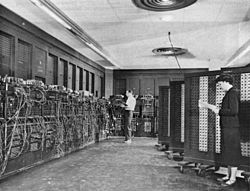
\includegraphics[width=4cm]{ENIAC.jpg}
\end{wrapfigure}
\historyFont 
ENIAC (Electronic Numerical Integrator And Computer) was one of the first general purpose computers. It was built during WW2 and completed in 1946. It was funded by the U.S. Army and was used to calculate ballistic tables for artillery shells, taking into account the effects of drag, wind and other factors influencing projectiles in flight. 

ENIAC, unlike the computers of today was a colossal machine, weighing 30 tons, consuming 150 kilowatt of power and taking up 1800 square feet of floor space. 

At the time it was proclaimed in the media as `a human brain'. 
It was very fragile and components needed frequent replacing. The first primary programmers of ENIAC were:

\centerline{
\begin{tikzpicture}[xscale=1.2]
	%
	\tikzstyle{p}=[text width=1.5cm]
	\tikzstyle{l}=[font=\smaller,align=center, fill=white,inner sep=1pt, draw,drop shadow]
	%
	\node[p] (P) {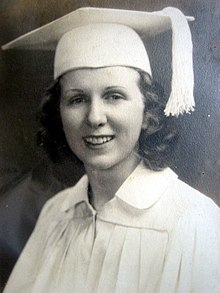
\includegraphics[width=\textwidth]{KayMcNulty.jpg}};
	\node[l] at ($(P.south)+(0,0)$) {Kay McNulty};
%
	\node[p] at (2,0) 
	(P) {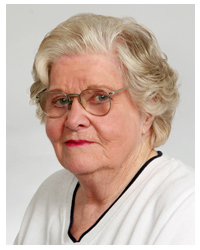
\includegraphics[width=\textwidth]{Jean_Bartik.jpg}};
	\node[l] at ($(P.south)+(0,0)$) {Jean Bartik};
%
	\node[p] at (4,0) 
	(P) {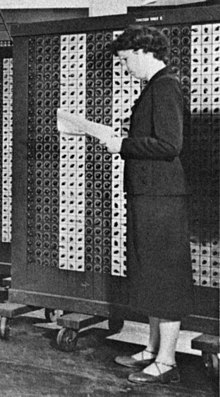
\includegraphics[width=\textwidth,clip,trim=0 100 0 0]{Betty_Holberton.jpg}};
	\node[l] at ($(P.south)+(0,0.2)$) {Betty\\ Holberton};
%	
	\node[p] at (6,0) 
	(P) {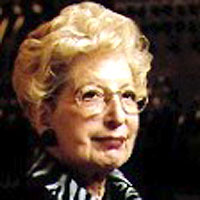
\includegraphics[width=\textwidth]{Marlyn_Meltzer.jpg}};
	\node[l] at ($(P.south)+(0,0)$) {Marlyn Meltzer};
%
	\node[p] at (8,0) 
	(P) {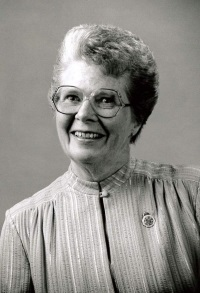
\includegraphics[width=\textwidth,clip,trim=0 50 0 0]{Frances_Spence.jpg}};
	\node[l] at ($(P.south)+(0,0)$) {Frances\\ Spence};
%
	\node[p] at (10,0) 
	(P) {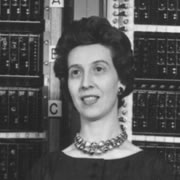
\includegraphics[width=\textwidth]{Ruth_Teitelbaum.jpg}};
	\node[l] at ($(P.south)+(0,0)$) {Ruth Teitelbaum};
\end{tikzpicture}}

%Kay McNulty, Betty Jennings, Betty Snyder, Marlyn Meltzer, Fran Bilas, and Ruth Lichterman were the first programmers of the ENIAC.

\end{tcolorbox}

\section{Throwing Up, or Dropping Down}

\subsection{Our First Experiment: Dropping a ball}


\tcbsidebyside[enhanced,lefthand width=5cm,
	attach boxed title to top center={yshift=-12pt},
	coltitle=black,boxed title style={colback=green!10},
	title=\bf Experiment One: Dropping Down,
	]{
\centerline{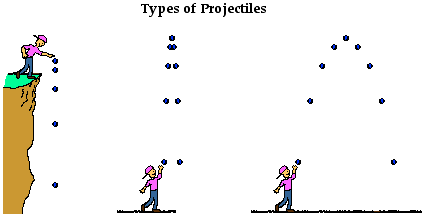
\includegraphics[scale=.8,clip,trim=0 0 350 20]{projectiles}}
}{
You are standing at the top of a tall cliff (height is 25 m) and you drop a ball. What we want to know is
\begin{itemize}
\item
How long will the ball take till it hits the ground? 
\item
How fast will the ball be moving when it hits the ground?
\item
How are you going to get your ball back?
\end{itemize}
}

We can't just say to our computer ``{\em Hey solve this problem for me!}'' we need to break this down and tell it how to solve this problem.  Like most computer problems this come down to asking ``What information do we need to store?'' ,  ``What calculations do we need to do?'', and finally ``What output do we wsnt to see?''

\vspace{6pt}
\tikz\node[fill=white,drop shadow,draw, signal] 
{{\sc Step 1:} What information do we need to store?};

\begin{itemize}
\item {\bf Position/Height of the ball.} We will use variable \code{y} for this. Yes, we could use \code{h} for height and it would make more sense here, but in general we tend to use \code{y} for vertical positions and \code{x} for horizontal positions.  Initially the ball is 25 metres above the ground so we write:

\codeonly{}{1}{1}{code}{Basic.py}    

\item {\bf Velocity of the ball.} We will use variable \code{v} for this.  Initially the ball is not moving so we write:

\codeonly{}{2}{2}{code}{Basic.py}    

\item {\bf Acceleration of the ball.} We will use variable \code{a} for this. When we release the ball, it will start moving downwards, due to the effect of gravity.  This `pull' effect feel like an acceleration and is approximately -9.81 $\text{m}/\text{s}{^2}$.  The minus sign is because it points downwards towards the ground. So we write:

\codeonly{}{3}{3}{code}{Basic.py}    

\item {\bf Time.} We will use variable \code{t} for this. And we are going to start measuring time from the instant we drop the ball. so we write:

\codeonly{}{4}{4}{code}{Basic.py}    

\item {\bf Time Step.} What is this? Think of the ball falling and we taking picture after picture of it as it falls. The computer will calculate the position and velocity at each picture. The more pictures we take the more calculations the computer will make but the more accurate our results will be. We want to take enough picture to get results that are `accurate enough' but not so much pictures the computer takes too long to do the calculations. Lets take ten pictures every second, so the time between pictures is 0.1, and we write

\codeonly{}{6}{6}{code}{Basic.py}    
\end{itemize}


\vspace{6pt}
\tikz\node[fill=white,drop shadow,draw, signal] 
{{\sc Step 2:} What calculations do we need to do?};\vspace{6pt}

We are going to keep taking picture after picture as the ball falls. To get the computer to repeat something for evert we write 

\codeonly{}{8}{8}{code}{Basic.py}  

At every `picture' we need to calculate the ball's position --- compare the code to equation~(\ref{eq:position})

\codeonly{}{10}{10}{code}{Basic.py}  

and the ball's velocity --- compare the code to equation~(\ref{eq:velocity})

\codeonly{}{11}{11}{code}{Basic.py}  

and update time. To update time we just add to our current value for time the time step. So we write

\codeonly{}{12}{12}{code}{Basic.py}  

Putting all of the above line together we get 

\codeonly{}{1}{12}{code}{Basic.py}  

\TODO{Create a new program with the above code and save it as  \code{Drop_1.py}.

Run the program, what happens?
}

In our current program the computer appears to be busy doing work but we see nothing! We\footnote{OK, OK, I forgot, but you should have reminded me that I forgot \ldots} forgot to do step 3 and tell the computer what information to output. Lets fix that now.

\clearpage
\vspace{6pt}
\tikz\node[fill=white,drop shadow,draw, signal] 
{{\sc Step 3:} What information do we want to output?};\vspace{6pt}

At every `picture' we take we are interested in the time the picture was taken and the position and the velocity of the ball. To do this  we append the following line to our program:
 
\codeonly{}{14}{14}{code}{Basic.py}  

Note the indentation in the above line. It is part of the \code{while} loop. Otherwise it will only output the final position and velocity.

\TODO{Append the above line to your \code{Drop_1.py} program and run it. What happens?}

It is a feast or a famine --- now we are drowning in data! There are two problems here:

\begin{itemize}
\item
The computer does not stop when the ball hits the ground --- think about this, why would the computer stop? how does it know about the ground? 

Remember, computers are fast but stupid --- we need to tell the computer when to stop.  In this experiment we want to break out of our \code{while} loop when the ball hits the ground, that is, when the height of the ball is zero, so we append line 

\codeonly{}{16}{16}{code}{Basic.py}  

Why did we use ``\code{y<0}'' and not ``\code{y==0}''?  In other words, why did we test if the height is less than zero instead of testing if the height is exactly zero?  

We did this because, when we take our pictures we are very, very unlikely to take the picture at the exact point in time at which the ball hits the ground so our test checks if the ball has hit the ground instead.

\item
What is the story with all the digits after the decimal point?  The computer does not know how accurate you want your output so it outputs as much accuracy as it can compute.  To fix this, change the print line from

\codeonly{}{14}{14}{code}{Basic.py}  
to
\codeonly{}{14}{14}{code}{Drop_1.py}  

This command is looks complicated but if we break it down it should become clearer:
\begin{itemize}
\item The code \code{"\%12.2f \%12.2f \%12.2f"} is called a {\bfseries format string}. Think of it as a message with three empty boxes in it. The data after the string is used to fill in each box.  
\item The letter ``\code{f}'' is used to say that the data will be a float (a number with a decimal point).
\item The ``12.2'' says to use at least 12 spaces to output the number but only output two digits after the decimal point.
\end{itemize}

\end{itemize}

\TODO{Run your updated program and answer the following questions, in the space provided.

\par{\bf Question:} How long is the ball falling? \hfill  \tikz\node[draw,text height=14pt,text width=3cm,align=right] {s};

\par{\bf Question:} At what speed is the ball moving when it hits the ground? \hfill  \tikz\node[draw,text height=14pt,text width=3cm,align=right] {$\text{m}/\text{s}$};
}


\clearpage

Our program works but there are some issues:
\begin{itemize}
\item We don't see the ball position and velocity AT the instant we drop the ball.  

This is easy --- just change the order of the compute lines with the print line.

\item We could improve our output by adding a message to label each column of data.

This is also easy --- we just insert a print command before the \code{while} loop.

\item We want to take more pictures but that will mean more output --- how can tell the computer compute more values but only output some of these?

This will require an \code{if} statement.
\end{itemize}
 
The following program fixes the above three issues.

\TODO{Create a new program with the following code and save it as  \code{Drop_2.py}.}

\codeonly{title={\code{Drop_2.py}}}{1}{40}{code}{Drop_2.py}

\begin{itemize}
\item
Notice the new variable \code{output_dt} and the \code{if} condition on line 17. These control how often we output results.  We can now make \code{dt} as small as we like (depending on how fast our computer is) to get more accurate results, but still only outputting the same amount of data.

\end{itemize}
\subsection{Our Second Expexriment: Throwing Up (without the mess!)}

\tcbsidebyside[enhanced,lefthand width=5cm,
	attach boxed title to top center={yshift=-12pt},
	coltitle=black,boxed title style={colback=green!10},
	title=\bf Experiment One: Dropping Down,
	]{
\centerline{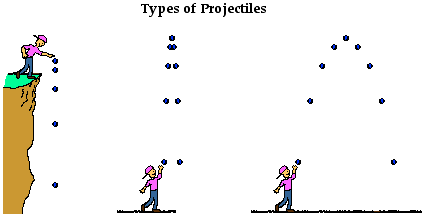
\includegraphics[scale=.8,clip,trim=150 0 200 20]{projectiles}}
}{
You throw a ball up into the air with an initial velocity of 25 m/s. What we want to know is
\begin{itemize}
\item
How long will the ball take till it hits the ground? 
\item
How fast will the ball be moving when it hits the ground?
\item
What is the maximum height that the ball reaches?
\end{itemize}

To keep everybody's results the same we are going to assume that your hand is 1.3 metres above the ground..
}

\TODO{Save your \code{Drop_2.py} program as \code{Throw_1.py} and modify it to look like the following.}

\codeonly{title={\code{Throw_1.py}}}{1}{40}{code}{Throw_1.py}


\TODO{The program runs but the maximum height is incorrect.  You need to insert some computation lines to update the maximum height, and then answer the following questions.

\par{\bf Question:} How long is the ball in the air? \hfill  \tikz\node[draw,text height=14pt,text width=3cm,align=right] {s};

\par{\bf Question:} At what speed is the ball moving when it hits the ground? \hfill  \tikz\node[draw,text height=14pt,text width=3cm,align=right] {$\text{m}/\text{s}$};

\par{\bf Question:} What is the maximum height of the ball? \hfill  \tikz\node[draw,text height=14pt,text width=3cm,align=right] {$\text{m}$};
}

\TODO{This task is a little harder.  Try it and we are here to help.

You need to modify the code so that it also stores when the ball reaches maximum height and then answer the following questions.

\par{\bf Question:} How long is the ball moving upwards? \hfill  \tikz\node[draw,text height=14pt,text width=3cm,align=right] {s};

\par{\bf Question:} How long is the ball moving downwards? \hfill  \tikz\node[draw,text height=14pt,text width=3cm,align=right] {s};

\par{\bf Question:} What is the total distance the ball moves? \hfill  \tikz\node[draw,text height=14pt,text width=3cm,align=right] {m};
}

\TODO{This task is a little harder again.  Try it and we are here to help.

\par\parbox{12cm}{{\bf Question:} At what velocity is the ball moving when it passes your hand on the way down?}\hfill  \tikz\node[draw,text height=14pt,text width=3cm,align=right] {m/s};
}


\subsection{Can I see it?}

Numbers are great and all that \ldots\ but a picture would be nice.  Lets use some turtle graphics to visualise our ball. To do this we 
\begin{itemize}
\item Lets call our turtle \code{ball} instead of \code{bob}, (but feel free to keep \code{bob} if you like) so we write

\codeonly{}{12}{13}{code}{Throw_2.py}

\item Since throwing a turtle is not nice, lets change it to a ball, so we write

\codeonly{}{14}{15}{code}{Throw_2.py}

\item Next we setup the ball's initial position using

\codeonly{}{17}{19}{code}{Throw_2.py}

\item And trance the ball movement using 

\codeonly{}{31}{31}{code}{Throw_2.py}

\end{itemize}

\TODO{Save your \code{Throw_1.py} program as \code{Throw_2.py} and modify it to look like the following.}

\codeonly{title={\code{Throw_2.py}}}{1}{50}{code}{Throw_2.py}

To be fair, that output was kinda sad. We need to zoom in a bit to see it properly. To do this is we insert two lines to create a screen where the x- and y- coordinates are more suited to our needs.

\TODO{Save your \code{Throw_2.py} program as \code{Throw_3.py} and insert the following two lines.}

\codeandoutput{title={\code{Throw_3.py} (only showing new lines) }}{12}{15}{code}{Throw_3.py}{

	\centering	
	\tikz\node[fill=white]{
	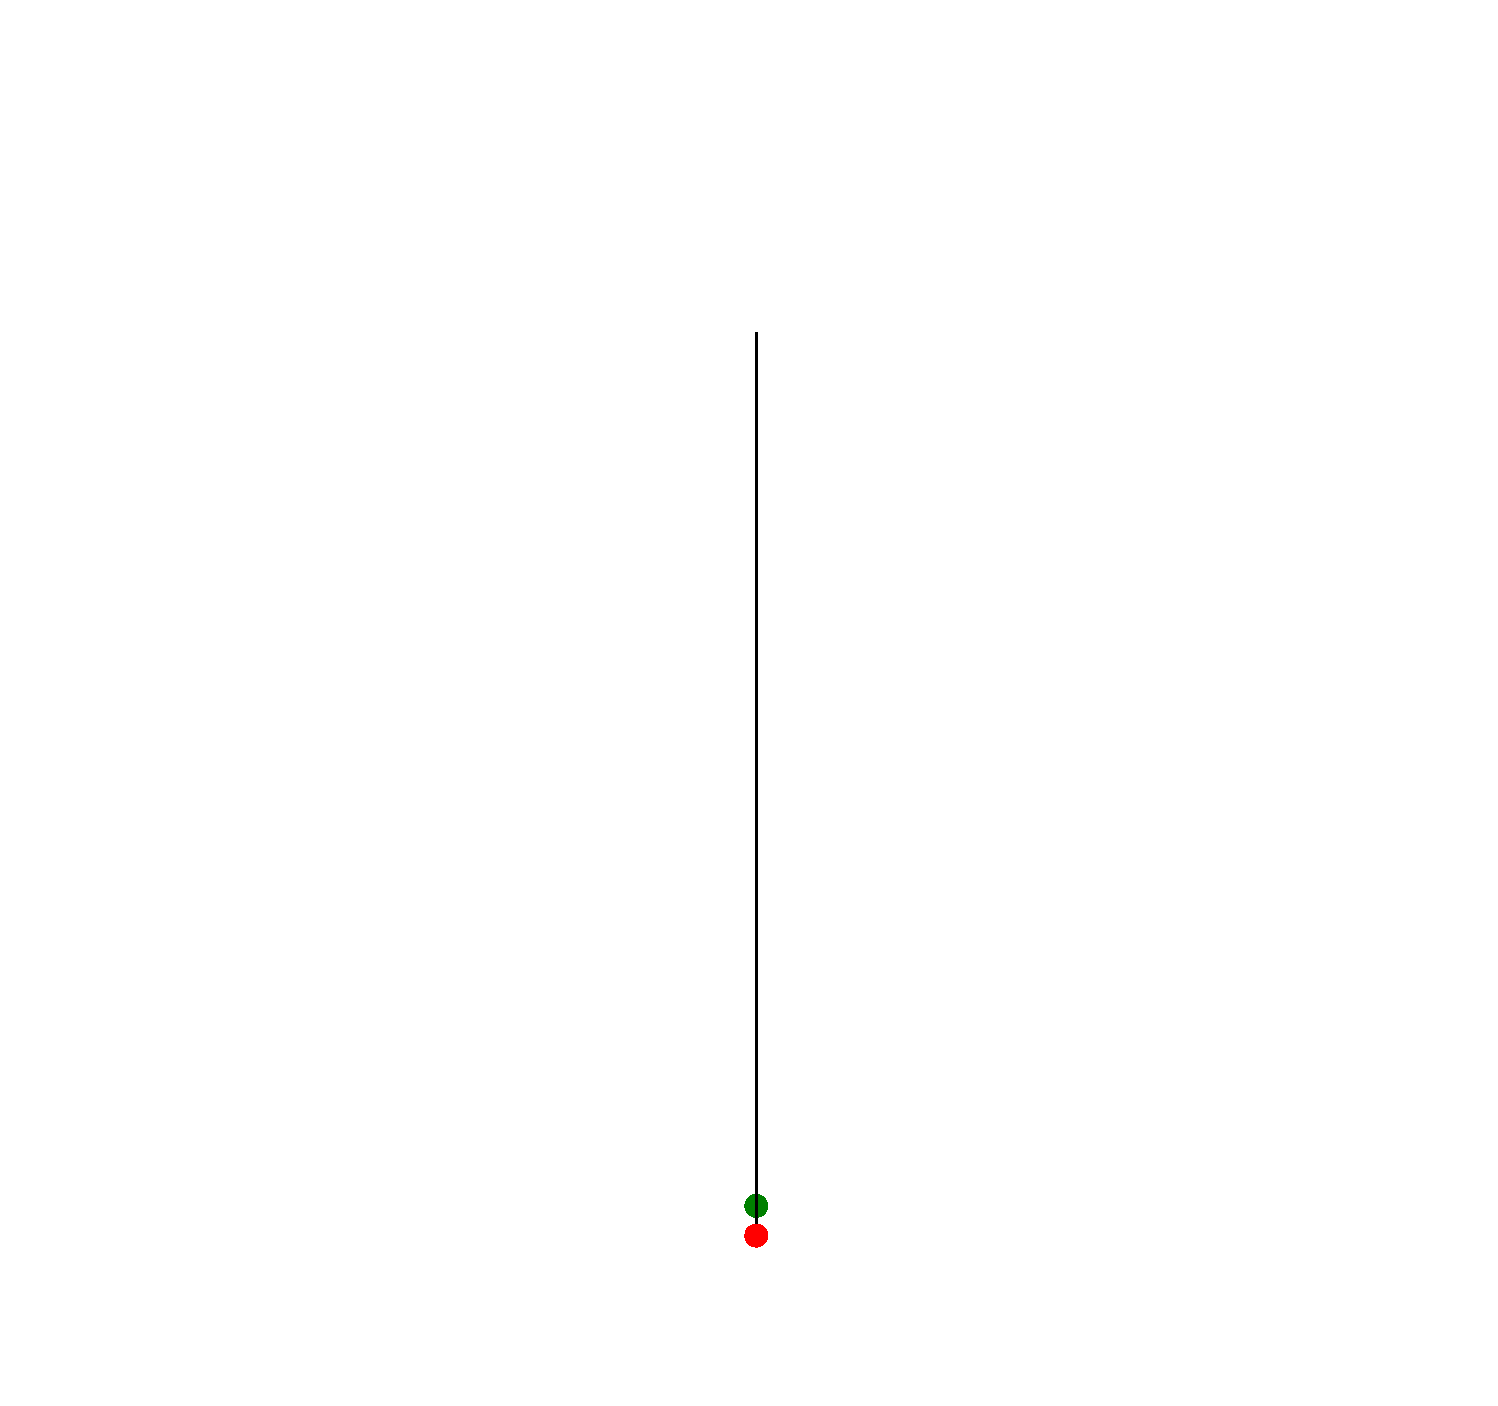
\includegraphics[clip,trim=0 10 0 10, width=\textwidth]{code/Throw_4.pdf}};
}

\TODO{
OK, this is a little better.  I have added some other to mark the start point as green and the end point as red. Modify your \code{Throw_3.py} code so that we see the start and the end point using the command
\code{ball.stamp()} and \code{ball.color()}.} 

\section{Where are we now?}

OK, we have done enough for today, next week we are going to:

\begin{itemize}
\item
Move to two-dimensional projectile movement.
\item 
Generate graphs of the projectile movement.
\end{itemize}
%\section{One Dimension is Boring, Lets go 2D}

\end{document}


